\documentclass[12pt,fleqn]{article}\usepackage{../../common}
\begin{document}
Temel Fizik 3, Basınç, Çarpışma

Elastik Çarpışma (Elastic Collision)

$m_1,m_2$ kütlesine sahip $v_1,v_2$ hızında iki küre arasında mükemmel bir
elastik çarpışma olduğunu düşünelim, yani çarpışma öncesi ve sonrası enerji
kaybı yok, bu durumda, sistemin toplam momentumu da önce ve sonra aynı
olacaktır, 

$$
m_1 \vec{v}_1 + m_2 \vec{v}_2 = m_1 \vec{v}_1' + m_2 \vec{v}_2' 
$$

ki $\vec{v}_1,\vec{v}_2,\vec{v}_1',\vec{v}_2'$ hız vektörleri,
$\vec{v}_1',\vec{v}_2'$ çarpışma sonrası hız vektörleri.

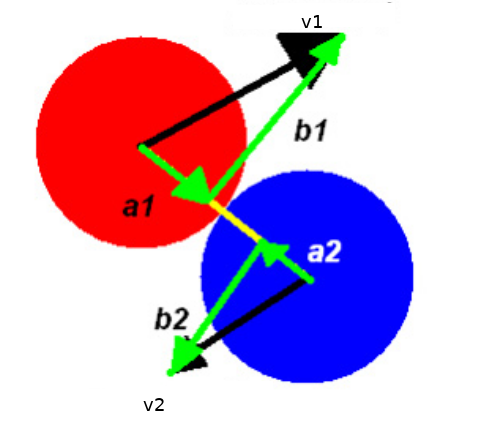
\includegraphics[width=20em]{phy_005_basics_06.png}

Eğer momentum muhafaza ediliyorsa, birinci topun kaybettiği ya da kazandığı
momentum ikinci topa eklenecek ya da ondan çıkartılacaktır.

$$
m_1 \vec{v}_1 = m_1 \vec{v}_1' - \Delta \vec{p}
$$

$$
m_2 \vec{v}_2 = m_2 \vec{v}_2' + \Delta \vec{p}
$$

Üstteki idealize ortamda momentum transferi sadece çarpışma çizgisi üzerinde
olabilir, bu çizgi, ya da vektör yönü eğer iki topun arasında teğet bir düzlem
düşünsek ona dik olan bir vektör olacaktır, ona $n$ diyelim. O zaman, ve $p$
vektörünün büyüklüğünü $P$ ile gösterirsek,

$$
\vec{v}_1' = \vec{v}_1 - (P / m_1) \vec{n}
\mlabel{1}
$$

$$
\vec{v}_2' = \vec{v}_2 + (P / m_2) \vec{n}
\mlabel{2}
$$

Eğer $P$ skalar büyüklüğünü bulabilirsek, çarpışma sonrası yeni hızı elde
edebiliriz. 

Üstteki resme bakınca görüyoruz ki $v_1$ ve $v_2$ her biri iki tane ayrı
vektörün toplamı olarak temsil edilebilir, bu vektörlerden biri çarpışma,
momentum transfer çizgisine dik, diğeri ona paralel. Bu bilgi ile,
$v_1,v_1',v_2,v_2'$ şöyle temsil edilebilir,

$$
\vec{v}_1 = a_1 \vec{n} + b_1 \vec{q}, \qquad \vec{v}_2 = a_2 \vec{n} + b_2 \vec{q}
\mlabel{3}
$$

$$
\vec{v}_1' = a_1' \vec{n} + b_1' \vec{q}, \qquad v_2' = a_2' \vec{n} + b_2' \vec{q}
\mlabel{4}
$$

$a_1,a_2,b_1,b_2$ tek sayı değerleridir. 

(1) formülüne (3a)'yı sokarsak,

$$
v_1' = a_1 \vec{n} + b_1 \vec{q} - (P/m_1) \vec{n}
$$

$$
 = (a_1 - p/m_1) \vec{n} + b_1 \vec{q}
$$


$$
v_2' = a_2 \vec{n} + b_2 \vec{q} + (P/m_2) \vec{n}
$$

$$
= (a_2 + P/m_2) \vec{n} + b_2 \vec{q}
$$

Ve tabii ki form olarak $\vec{v}_1' = a_1' \vec{n} + b_1' \vec{q}$, ve
$\vec{v}_2' = a_2' \vec{n} + b_2' \vec{q}$ olduğunu biliyoruz, o zaman birbirine
tekabül eden kısımlara bakarak

$$
a_1' = a_1 - (P/m_1), \qquad b_1' = b_1
\mlabel{5}
$$

$$
a_2' = a_2 + (P/m_2), \qquad b_2' = b_2
\mlabel{6}
$$

Şimdi $P$ tek sayı değerini bulmak için enerji muhafazası formülünü
kullanabiliriz. Tek boyutta $1/2 m v^2$ şeklinde olan formülü $\frac{1}{2} m
\cdot \vec{v}\cdot\vec{v}$ olarak değiştirmek lazım. Ya da $\frac{1}{2} m
<\vec{v},\vec{v}>$, ya da $\frac{1}{2} m ||v||^2$.  O zaman

$$
\frac{m_1}{2} ||v_1||^2 + \frac{m_2}{2} ||v_2||^2  =
\frac{m_1}{2} ||v_1'||^2 + \frac{m_2}{2} ||v_2'||^2 
$$

$||v_1||^2$ ve $||v_1'||^2$, vs hesabının kolay bir yolu var, eğer üstteki resme
bakarsak mesela $||v_1||$ büyüklüğü kenarları $a_1$ ve $b_1$ olan bir üçgenin
hipotenüsü olarak görülebilir.

$$
\frac{m_1}{2} (a_1^2+b_1^2) + \frac{m_2}{2} (a_2^2+b_2^2) =
\frac{m_1}{2} (a_1'^2+b_1'^2) + \frac{m_2}{2} (a_2'^2+b_2'^2) 
$$

Daha önce bulduğumuz (5),(6) değerlerini üstteki formüle sokunca,

$$
\frac{m_1}{2} (a_1^2+b_1^2) + \frac{m_2}{2} (a_2^2+b_2^2) =
\frac{m_1}{2} \left( \left(a_1-\frac{P}{m_1} \right)^2 + b_1^2 \right)  +
\frac{m_2}{2} \left( \left(a_2-\frac{P}{m_1} \right)^2 + b_2^2 \right) 
$$

$b_1^2$ ve $b_2^2$ iptal olur. Her şeyi $P$ sol tarafta olacak şekilde tekrar
düzenlersek,

$$
P = \frac{2 m_1 m_2 (a_1-a_2)}{m_1+m_2}
$$


Bu degeri (1) ve (2)'ye sokarsak,


$$
\vec{v}_1' = \vec{v}_1 - \frac{2 m_2 (a_1-a_2)}{m_1+m_2} \vec{n}
$$

$$
\vec{v}_2' = \vec{v}_2 + \frac{2 m_1 (a_1-a_2)}{m_1+m_2} \vec{n}
$$

Üstteki formülü değişik kaynaklarda, mesela [3], biraz farklı formda görüyoruz,
mesela

$$
\vec{v}_1' =
\vec{v}_1 - \frac{2m_2}{m_1+m_2}
\frac{< \vec{v}_1-\vec{v}_2, \vec{x}_1-\vec{x}_2 >}{||\vec{x}_1-\vec{x}_2||^2}
(\vec{x}_1-\vec{x}_2)
$$

$$
\vec{v}_2' =
\vec{v}_2 - \frac{2m_1}{m_1+m_2}
\frac{< \vec{v}_2-\vec{v}_1, \vec{x}_2-\vec{x}_1 >}{||\vec{x}_2-\vec{x}_1||^2}
(\vec{x}_1-\vec{x}_2)
$$

Fakat biraz dikkat edilince mesela $a_1-a_2$'nin $\vec{n}$ yönündeki hız farkı
olduğunu görürüz, yani

$$
a_1-a_2=\frac{< \vec{v}_1-\vec{v}_2,\vec{x}_1-\vec{x}_2 >}{||\vec{x}_1-\vec{x}_2||}
$$

Geri kalanlardan zaten $\vec{n} = \vec{x}_1-\vec{x}_2/||\vec{x}_1-\vec{x}_2||$
ve $m_1,m_2$ değerleri de aynı şekilde iki tarafta uyar.

İki kütlenin eşit olduğu durumlarda (ki moleküler simülasyonlarda bu çok rahat
kabul edilebilir), formül daha da basitleşir [4],

$$
v_1' = v_1 - \left( (v_1-v_2)  \cdot \vec{n} \right) \vec{n}
$$

$$
v_2' = v_2 - \left( (v_2-v_1)  \cdot \vec{n} \right) \vec{n}
$$

ki $\vec{n} = \frac{x_1-x_2}{|x_1-x_2|}$

Basınç (Pressure)

Bir sıvı içinde duran bir objeye tek uygulanan etki, stres onu
sıkıştıran türden bir etkidir. Diğer bir deyişle bir sıvı içindeki
objenin hissettiği kuvvet onun yüzeyine her zaman diktir.

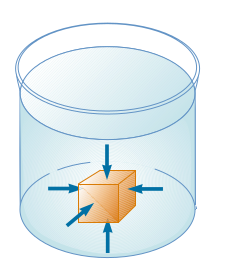
\includegraphics[width=10em]{phy_005_basics_07.png}

Bir sıvının içindeki objeye uyguladığı basıncı, o objeye uygulanan
birim alanda uygulanan kuvvet olarak temsil edilebiliriz, kuvvet $F$
ve alan $A$ ise,

$$
P \equiv \frac{F}{A}
$$

Eğer belli bir noktadan bahsetmek istersek, diyelim $dA$ sonsuz
ufaklıktaki bir alana uygulanan $dF$ kuvveti,

$$
P = \frac{dF}{dA}
$$

O zaman belli bir alandaki basınç için o alan üzerinden entegral almak gerekir. 

Basıncın birimi $N / m^2$, şaşırtıcı olmasa gerek, kuvvet birimi
Newton, ve alan birimi $m^2$.

İdeal Gazlar Kanunu (İdeal Gas Law)

Peki mikro etkileşimlerden yola çıkarak basınç kavramını türetebilir miyiz
acaba? 19'uncu yüzyıl sonlarına doğru bu başarıldı ve gerçekten temel mekanik
kanunlarının basit bir model üzerinen makro açıklamalar yapabilmesinin çok güzel
bir örneği.

Basıncın gaz moleküllerinin bir yüzeye çarpmasından ortaya çıktığını
hatırlayalım. Bu kuvvet tabii ki Newton kanunundan hareketle,

$$
f = m a = m \frac{\ud v}{\ud t}
$$

Hız $v$'ye molekül içinde olduğu kabin / yüzey duvarına çarptığında ona dik olan
hız diyelim [1]. Bu türevi hesaplamak için, ki birim zamanda hız değişimi
gerekiyor, kenarları $L$ uzunluğunda bir küp içinde tek bir gaz molekül olduğunu
düşünelim.

Basitleştirme amacıyla diyelim ki bu molekül sürekli küp kutu içinde ileri geri
gidip geliyor, bir duvara çarpınca bir süre sonra geri geliyor. Bu molekül bir
duvara çarptığında $v$ hızında çarptığında (yani $mv$ momentumuyla) elastik
olarak geri sekecektir, ve $-v$ ile tam ters yöne geri gitmeye başlayacaktır.

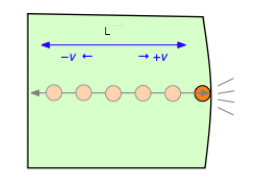
\includegraphics[width=20em]{phy_005_basics_04.png}

O zaman her çarpışma için hız değişimi $2v$, momentum değişimi ise $2mv$
olur.

Tabii aslında eğer daha genel formülize etmek gerekirse bu çarpışma sırasında
$\bar{v}$ hızının duvara dik olan bileşeni $v_x$'yi düşünüyoruz.

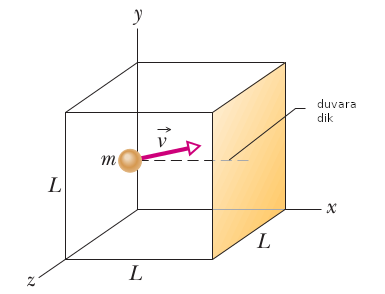
\includegraphics[width=20em]{phy_005_basics_05.png}

Yani momentum degisimi

$$
\Delta p_x = (-m v_x) - (m v_x) = - 2 m v_x 
$$

Yani duvara transfer edilen momentum $2 m v_x$. 

Birim zaman $\Delta t$'ye bir molekün iki çarpışma arasında geçen zaman dersek,
ve $v_x$ hızında $2L$ yol katedilmişse, $\Delta t  = 2 L / v_x$ demektir, ve

$$
F = \frac{\Delta p_x}{\Delta t} = \frac{2 m v_x}{2 L / v_x} = \frac{m v_x^2}{L}
$$

Basınç birim alana uygulanan kuvvettir, ve küpün bir kenarının $L^2$ alaninda
olduğunu düşünürsek, 

$$
P = \frac{m v^2}{L^3} = \frac{m v^2}{V}
$$

$V$'yi kutunun hacmi olarak aldık, ve $V = L^3$.

Birden fazla molekülü düşünmek istiyoruz şimdi, mesela bir averaj
üzerinden.. Fakat her molekül hem negatif hem pozitif yönde aşağı yukarı aynı
miktarda hareket yapar (rasgele hareket olduğu için) ve bu tür bir hareket
üzerinden averaj almak bizi sıfır değerine götürür. Bu sebeple ortalamasını
almadan önce hızların karesini almak istiyoruz,

$$
\bar{v^2} = \frac{v_1^2 + v_2^2 + ... + v_N^2 }{N} = \frac{\sum_i v_i^2}{N}
$$

ve ortalama değeri bulmak için $\sqrt{\bar{v^2}}$ kullanıyoruz. Bu hesaba kök
kare ortalaması (root mean square -RMS-) ismi de verilir. Şimdi tüm $N$
moleküller üzerinden bir basınç hesaplamak istersek, $N$ tane molekül, ama belli
bir anda sadece Kartezyen kordinat sisteminde sadece üç yönden sadece biri
yönünde etki var, o zaman $N$ ile çarpıp 3'e bölmek lazım, 

$$
P = \frac{N}{3} \frac{m \bar{v^2}}{V}
$$

Bu formül içinde bir kinetik enerji formülasyonu görülebiliyor, averaj kinetik
enerjiye $\epsilon = m \bar{v^2} / 2$ dersek, üstteki formülü

$$
PV = \frac{N}{3} m \bar{v^2} = \frac{2}{3} N \epsilon
$$

olarak yazabiliriz.

Eğer bu formülü sıcaklık içerek şekilde değiştirmek istiyorsak; biliyoruz ki
sisteme eklenen her Joule enerji ve bir derece sıcaklık değişimi arasındaki
ilişkiyi $k$ sabiti kontrol eder [5, 29-16] bu sabit $k = 1.38 x 10^{23}$ Joule
/ Kelvin'dir, o zaman enerjiden sıcaklığa geçiş için $kT$ kullanabiliriz, hatta
bir $3/2$ eklenerek üstteki 2/3 iptali amaçlanır,

$$
\epsilon = \frac{3}{2} k T
$$

Ve,

$$
PV = \left( \frac{2}{3} N \right) \left( \frac{3}{2} k T \right) = N k T
$$

Devam edelim, $n = N / N_A$ olduğunu da biliyoruz ki $N_A = 6.02 x 10^{23}$,
Avagadro'nun sayısı, $n$ örneklemdeki mol sayısı, $N$ ise örneklemdeki tüm
moleküller [2, sf. 550],

$$
PV = n N_A k T
$$

Tabii bu bizi $R$ denen bir diğer sabite götürüyor, $R = 8.31 J/mol \cdot
K$. Onun $k$ ve $N_A$ ile ilişkisi şöyle,

$$
k = \frac{R}{N_A}
$$

O zaman,

$$
PV = n R T
$$

İdeal gazlar kanununa erişmiş olduk.

Kaynaklar

[1] Chang, {\em Physical Chemistry for the Biosciences},
    \url{https://chem.libretexts.org/@go/page/41408}

[2] Resnick, Fundamentals of Physics, 10th Ed

[3] Wikipedia, {\em Elastic collision}, \url{https://en.wikipedia.org/wiki/Elastic_collision}

[4] Masson, {\em Elastic Collisions in 3D}, \url{https://exploratoria.github.io/exhibits/mechanics/elastic-collisions-in-3d/index.html}

[5] Feynman, {\em Feynman Lectures on Physics, I}

\end{document}
